\documentclass[conference, a4paper]{IEEEtran}
\usepackage{blindtext, graphicx, url}
\hyphenation{}


 %%% JS %%%
%Define the listing package
\usepackage{listings} %code highlighter
\usepackage{color} %use color
\definecolor{mygreen}{rgb}{0,0.6,0}
\definecolor{mygray}{rgb}{0.5,0.5,0.5}
\definecolor{mymauve}{rgb}{0.58,0,0.82}

%Customize a bit the look
\lstset{ %
backgroundcolor=\color{white}, % choose the background color; you must add \usepackage{color} or \usepackage{xcolor}
basicstyle=\footnotesize, % the size of the fonts that are used for the code
breakatwhitespace=false, % sets if automatic breaks should only happen at whitespace
breaklines=true, % sets automatic line breaking
captionpos=b, % sets the caption-position to bottom
commentstyle=\color{mygreen}, % comment style
deletekeywords={...}, % if you want to delete keywords from the given language
escapeinside={\%*}{*)}, % if you want to add LaTeX within your code
extendedchars=true, % lets you use non-ASCII characters; for 8-bits encodings only, does not work with UTF-8
frame=single, % adds a frame around the code
keepspaces=true, % keeps spaces in text, useful for keeping indentation of code (possibly needs columns=flexible)
keywordstyle=\color{blue}, % keyword style
% language=Octave, % the language of the code
morekeywords={*,...}, % if you want to add more keywords to the set
rulecolor=\color{black}, % if not set, the frame-color may be changed on line-breaks within not-black text (e.g. comments (green here))
showspaces=false, % show spaces everywhere adding particular underscores; it overrides 'showstringspaces'
showstringspaces=false, % underline spaces within strings only
showtabs=false, % show tabs within strings adding particular underscores
% stepnumber=1, % the step between two line-numbers. If it's 1, each line will be numbered
stringstyle=\color{mymauve}, % string literal style
tabsize=2, % sets default tabsize to 2 spaces
title=\lstname % show the filename of files included with \lstinputlisting; also try caption instead of title
}
%END of listing package%

\definecolor{darkgray}{rgb}{.4,.4,.4}
\definecolor{purple}{rgb}{0.65, 0.12, 0.82}

%define Javascript language
\lstdefinelanguage{JavaScript}{
keywords={typeof, new, catch, function, return, null, catch, switch, var, if, in, while, do, else, case, break, for},
keywordstyle=\color{blue}\bfseries,
ndkeywords={class, export, boolean, throw, implements, import, this, true, false, Math},
ndkeywordstyle=\color{darkgray}\bfseries,
identifierstyle=\color{black},
sensitive=false,
comment=[l]{//},
morecomment=[s]{/*}{*/},
commentstyle=\color{purple}\ttfamily,
stringstyle=\color{red}\ttfamily,
morestring=[b]',
morestring=[b]"
}

\lstset{
language=JavaScript,
extendedchars=true,
basicstyle=\footnotesize\ttfamily,
showstringspaces=false,
showspaces=false,
tabsize=2,
breaklines=true,
showtabs=false,
captionpos=b
}

 %%% END JS %%%


\begin{document}
\title{How does the implementation of\\
Strategy design pattern in JavaScript\\
affect Maintainability as measured by W}
\author{\IEEEauthorblockN{Oskar Ther\'{e}n}
\IEEEauthorblockA{Computer Engineering\\
The Institute of Technology at Link\"{o}ping University\\
Email: oskth878@student.liu.se}}

\maketitle

\begin{abstract}
\end{abstract}

\section{Introduction}
\label{sec:Introduction}
It is widely acknowledged among object-oriented programmers that design patterns are useful to solve commonly occurring problems within a given context when coding. Design patterns was mainly introduced to software developers through the Gang of Four that came out with the idea in their book from 1995~\cite{bibitem:GoF} the idea originaly came from an architectural concept. and since then they have been widely discussed and used.

Even though they are so popular there are few empirically justified reasons to use them according to C. Zhang and D. Budgen in their article ``What Do We Know about the Effectiveness of Software Design Patterns?''~\cite{bibitem:Zhang}.

The purpose of this report is to find out if the implementation of a specific design pattern, strategy [section~\ref{sec:Strategy}], will affect maintainability [section~\ref{sec:Maintainability}] in a positive way.
\\
\subsection{Research Question}
\begin{itemize}
	\item How does the implementation of Strategy design pattern in JavaScript affect Maintainability as measured by W
\end{itemize}
\subsection{Strategy design pattern}
\label{sec:Strategy}
\begin{figure}[ht!]
	\centering
	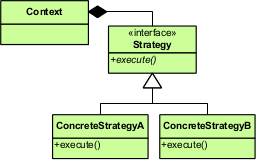
\includegraphics[scale=0.7]{Strategy_Pattern_in_UML.png}
	\caption{Strategy pattern in a UML-diagram}
	\label{fig:Strategy}
\end{figure}
Strategy is a behavioral pattern that intends to handle polymorphism by encapsulating a family of algorithms and make them interchangeable by abstracting away the algorithms different functionalities into separate classes that implements a common interface, which is called strategy. An UML-diagram over the concept is shown in [Figure \ref{fig:Strategy}]
\\
\subsection{SOLID}
The purpose of many design patterns is to solve some of the SOLID-violations that can arise when working on bigger projects. SOLID is an mnemonic acronym that stands for
\begin{itemize}
    \item Single responsibility \\
    Each class should only have responsibility over one part of the softwares functionality.
    \item Open-closed \\
    Classes, functions and so on, should be open for extension but closed for modification.
    \item Liskov substitution \\
    Every subtype should be able to replace its inherited type.
    \item Interface segregation \\
    Clients should not be forced to implement methods from and interface that it will not use.
    \item Dependency inversion \\
    High level modules should not be affected by changes of low level modules.
\end{itemize}
All of these principles are good to follow when developing software and are all contributing to code that is easier to maintain~\cite{bibitem:Bob}.

Strategy pattern mainly improves the code with Single responsibility and Open-closed in aspect, although it follows the other two principles as well.

\textit{Single Responsibility} through having the code for the algorithms in separate classes.

\textit{Open-closed} trough when adding a new algorithm the other code will not have to be changed, just add a new class for that algorithm and extend the interface.
\\
\subsection{Maintainability}
\label{sec:Maintainability}
The total cost of maintenance in software development is widely discussed and different eminent names in software development have claimed that it will take up from 40 even up to 60 percent of the time and cost to maintain a project. In the 1990s it was claimed by two experts, Corbi and Yourdon, that software maintainability where going to be one of the major challenges for the 1990s. During the 90s this was confirmed by Hewlett-Packard that claimed that ``they had between 40 and 50 million lines of code under maintenance and that 60 to 80 percent of research and development personnel are involved in maintenance activities''~\cite{bibitem:MetricsToEvaluate}.
\\
\subsection{Metrics}
There are several metrics that tries to measure the complexity of a function or a program. There are a lot of different advancement levels of these metrics, they can range from just lines of code to Robillards interconnectivity metric that ``integrates the structural as well as the textual aspects of a program in such a way that the organization of a program can be seen graphically. The measure of complexity depends on how a statement is related to the rest of the program''~\cite{bibitem:Robillard}.

Since the 1990s there have been several attempts to link maintainability with different metrics. In the article Using Metrics to Evaluate Software System Maintainability they found that when they conducted automated software maintainability analysis on 11 softwaresystems. They all corresponded to the experts intuition and also provided additional useful data~\cite{bibitem:MetricsToEvaluate}.

Wei and Henry came to similar conclusion when studing Object-Oriented Metrics that Predict Maintainability~\cite{bibitem:WeiHenry}.
\\
\section{Method}
safa
\\
\subsection{Interpretation of the Strategy pattern for JavaScript}
Firstly, since JavaScript is not an object oriented language the concept of interface does not exist. In Harmes et al. book ``Pro JavaScript\texttrademark~Design Patterns''~\cite{bibitem:DiazHarmes} the recommendation is to create a Duck Typed interface emulation. This would be useful if the Strategy pattern where used in a real life program to ensure correct parameters where sent to the functions. But since this reports purpose is to evaluate Strategy pattern and uses a quite small example and since JavaScript is loosely typed the implementation of an interface is skipped and type correctness is assumed.
\\
The example used in this report is taken from an existing game. The code that is supposed to be replaced with the Strategy pattern is a switch case that sets a \texttt{message} dependent on an enumerate:
\begin{lstlisting}[language=JavaScript, label=lst:switch-case, caption=The original switch case.]
switch(entity.objectType) {
	case ObjectTypeEnum.BUG:
		message = ...
		break;
	case ObjectTypeEnum.DROP:
		message = ...
		break;
	case ObjectTypeEnum.COLLECTABLE:
		message = ...
		break;
}
\end{lstlisting}
The goal is to replace this code with the following calls:
\begin{lstlisting}[language=JavaScript, label=lst:switch-case, caption=Switch case replaced trough the Strategy pattern.]
	var messager = new Messager(entity.objectType);
	message = messager.getMessage(message, ...);
\end{lstlisting}
This is very similar to how the call would look like in Java, the difference is that \texttt{messager} would be the type \texttt{Messager}.
\section{Result}
safa
\\
\section{Discussion}
aspjfa
\\
\section{Conclusion}
The conclusion goes here.

\clearpage
\begin{thebibliography}{1}
\bibitem{bibitem:GoF}
Erich Gamma, Richard Helm, Ralph Johnson and John Vlissides, \emph{Design Patterns: Elements of Reusable Object-Oriented Software}, \hskip 1em plus 0.5em minus 0.4em\relax Addison-Wesley Professional, 1st edition, January 15, 1995
\bibitem{bibitem:Zhang}
Cheng Zhang and David Budgen, \emph{What Do We Know about the Effectiveness of Software Design Patterns?}, \hskip 1em plus 0.5em minus 0.4em\relax IEEE Transactions on Software Engineering, vol. 38, no. 5, pp. 1213-1231, September-October 2012
\bibitem{bibitem:Bob}
Robert C.~Martin, \emph{Principles Of OOD}, \hskip 1em plus 0.5em minus 0.4em\relax \url{http://butunclebob.com/ArticleS.UncleBob.PrinciplesOfOod}, Accessed: 2015-10-17, Dates back to at least 2003
\bibitem{bibitem:MetricsToEvaluate}
Don Coleman, Dan Ash, Bruce Lowther and Paul Oman, \emph{Using Metrics to Evaluate Software System Maintainability}, \hskip 1em plus 0.5em minus 0.4em\relax Computer, Volume:27,  Issue: 8, August, 1994
\bibitem{bibitem:Robillard}
Pierre N.~Robillard and Germinal Boloix, \emph{The Interconnectivity Metrics: A New Metric Showing How a Program Is Organized}, \hskip 1em plus 0.5em minus 0.4em\relax Journal of Systems and Software, Volume 10, Issue 1, July 1989, Pages 29-39
\bibitem{bibitem:WeiHenry}
Wei Li and Sallie Henry, \emph{Object-Oriented Metrics that Predict Maintainability}, \hskip 1em plus 0.5em minus 0.4em\relax Journal of Systems and Software, Volume 23, Issue 2, November 1993, Pages 111-122
\bibitem{bibitem:DiazHarmes}
Dustin Diaz and Ross Harmes, \emph{Pro JavaScript design patterns}, \hskip 1em plus 0.5em minus 0.4em\relax Apress, 2008

\end{thebibliography}

\end{document}
